% textidote: ignore begin
\section{Large language model implementation}\label{sec:large-language-model-implementation}
% textidote: ignore end

As mentioned in Section~\ref{subsec:must-haves}, some key features, hereby explanations and interactivity, are not
implemented in the first release of the ChessTeacher project.
This makes for an application that in the current state may not suffice to resolve the problem statement.
There are several reasons for this gap and this section will discuss a possible solution to this issue.

Artificial intelligence (AI) has seen a significant increase in popularity in recent years, with the development of
large language models (LLMs) being one of the most notable advancements.
LLMs provide a way to generate human-like text, which can be used in a variety of applications, with chatbots being a
popular example.
As the core concept of this project is replacing a human chess coach with a computer, LLMs could be a valuable addition.

A potential use case for an LLM in the project could be to provide explanations for the moves suggested by Stockfish.
Currently, the user is given the three best moves without any explanation as to why they are the best.
By using an LLM, the user could ask follow-up questions to the feedback, and the LLM could provide a more detailed
explanation.
An example of this interaction can be seen in Figure~\ref{fig:llm}.

% textidote: ignore begin
\begin{figure}[H]
    \centering
    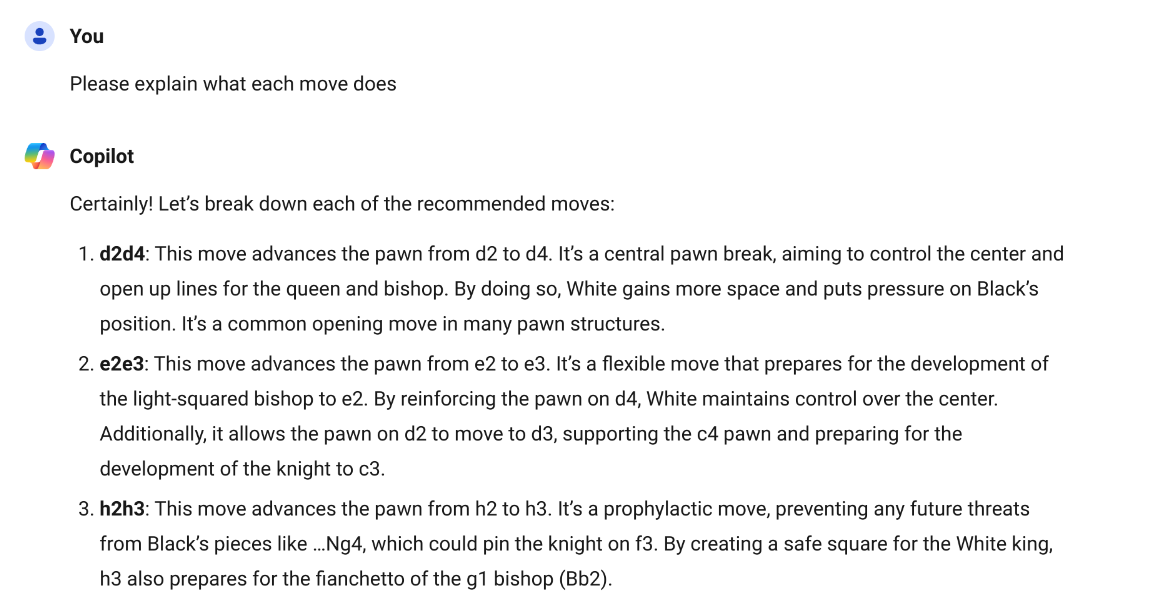
\includegraphics[width=0.85\textwidth]{llm}
    \caption{Example of a conversation with an LLM.}\label{fig:llm}
\end{figure}
% textidote: ignore end

It is important to note that LLM models are not perfect, and there are some potential issues that could arise from
implementing one.
The main concern is that the LLM could provide incorrect information, which could be detrimental to the learning
experience.
ChatGPT, a popular LLM, is known for its inability to actually play chess, as it often makes illegal
moves~\cite{llm-chess}.
The team however believes that Stockfish could be used in conjunction with the LLM to ensure that the information
provided is correct.
That would solve the issue of incorrect information, but it would also require a substantial amount of work.

The team did consider using an LLM during the planning phase of the project, but ultimately decided against it.
The main reason was because the team expected that Stockfish would provide a sufficient level of interactivity for the
users.
However, as evident from the usability testing results in Section~\ref{sec:results}, the feedback from Stockfish was
not able to contribute to the learning experience as much as the team had hoped.
Reflecting on this, the team believes that an LLM could be a valuable addition to the project, and should be implemented
if the project were to be expanded.
